% Definition des noms de la fonction
\newcommand{\frenchname}{Transfert d'eau dans le réseau hydrographique selon la méthode de propagation d'Hayami}
\newcommand{\englishname}{Water transfer on ditch network using hayami propagation method}

% Definition FileID
\newcommand{\FileID}{water.surf.transfer-rs.hayami}

% Definition variables produites
\newcommand{\VarProdA}{water.surf.Q.downstream-rs}
\newcommand{\VarProdB}{water.surf.H.level-rs}

% Used variables (if necessary)
\newcommand{\VarUsedA}{water.surf.Q.downstream-su}
\newcommand{\VarUsedB}{water.sz-surf.Q.baseflow}
\newcommand{\VarUsedC}{water.uz.Q.interflow}

% Definition parametres
\newcommand{\ParamA}{maxsteps}
\newcommand{\ParamB}{meancel}
\newcommand{\ParamC}{meansigma}
\newcommand{\ParamD}{calibstep}
\newcommand{\ParamE}{rsbuffer}

%Definition des proprietes distribuees
\newcommand{\PropDisA}{nmanning}
\newcommand{\PropDisB}{length}
\newcommand{\PropDisC}{width}
\newcommand{\PropDisD}{height}
\newcommand{\PropDisE}{slope}

% Main file for function description and utilisation


\selectlanguage{english}

\begin{abstract}
\iflanguage{english}{The ``\englishname'' compute the water transfer through the ditch network 
using the diffusive wave model resolved by the Hayami method. First, it 
calculates the input volume in reach segments. Then, the input hydrogram is 
convoluted using diffusive wave model with celerity and diffusivity as main 
parameters. Finally, the simulator converts the calculated output discharge 
to water height in the ditch using Manning-Strickler equation.
}{La fonction ``\frenchname'' réalise le transfert de l'eau à travers le réseau de fossés selon le modèle de propagation d'onde résolue par la méthode d'Hayami. Tout d'abord, elle calcule le débit entrant dans le tronçon. L'hydrogramme d'entrée est ensuite convolué selon le modèle de l'onde diffusante dont les principaux paramètres sont la célérité et la diffusivité de l'onde. Enfin, la fonction convertit le débit calculé en hauteur d'eau dans le tronçon selon l'équation de Manning-Strickler.}
\end{abstract}

%******************************
% Scientific concepts
\iflanguage{english}{\section{Scientific concepts}}{\section{Concepts scientifiques}}
\iflanguage{english}{\subsection{Calculation of input water discharge}
The simulator transfers water in hydrographic channel from upstream RS to discharge system RS. At each node, upper hydrograms are cumulated and propagated to downstream RS.

\includegraphics[width=8cm]{doc/common/Schema_GU_RS_SU_Hayami_RS.pdf}

The first step consists in computing the input discharge at the inlet of the ditch. This value is composed with discharge from potential connected RS or SU and subsurface and aquifer drainage flow if the model previously produces these variables. The equation is the following :

\begin{equation}
\label{InputDischarge}
Q_{in} = \sum_{RS_{Up}} Q_{RS} + \sum_{SU_{Up}} (Q_{SU} + Q_i) + \sum_{GU_{Up}} Q_b
\end{equation}


where $Q_in$ is the input water discharge at the inlet of the RS ($m\up3/s$), $Q_{RS}$ is the discharge produced by the upper connected RS, $Q_{SU}$ is the discharge from the upper SU, $Q_b$ is the baseflow discharge from connected GU ($m\up3/s$), and $Q_i$ is the interflow discharge ($m\up3/s$).\\


\subsection{Propagation using Hayami kernel}
Then, the input water discharge previously calculated is propagated between the gravity center of the main SU and the downstream unit. The propagation is done using the diffusive wave model \cite{Moussa1997} :

\begin{equation}
\frac{\delta Q}{\delta t} = -C \times \frac{\delta Q}{\delta x} + D \delta \frac{\delta \up2 Q}{\delta x\up2}
\end{equation}




In the particular case where wave celerity and diffusivity are constant, the diffusive wave equation can be resolved using an analytical solution \cite{Moussa1996}. The water output discharge is calculated using the following equation :

\begin{equation}
\label{HayamiConvolution}
Q_{RS}(t) = Q_{in}(t) * K(t)
\end{equation}




where $Q_{RS}$ is the produced output water discharge ($m\up3/s$), $Q_{in}$ is the input water discharge on RS ($m\up3/s$) calculated in the equation \ref{InputDischarge}, $*$ is the convolution product, and $K(t)$ is the ``Hayami kernel'' function expressed as :

\begin{equation}
K(t) = \frac{L}{2 \times (\pi D)^{\frac{1}{2}}} \times \frac{\text{exp}^{\frac{CL}{4D} \times \left(2-\frac{L}{Ct}- \frac{Ct}{L} \right) } }{t^{\frac{3}{2}}}
\end{equation}




where $L$ is the length of RS ($m$), $D$ is the wave diffusivity ($m\up2/s$), and $C$ is the wave celerity ($m/s$).\\

To resolved the equation \ref{HayamiConvolution}, the simulator temporarily sweeps the Hayami kernel. $\tau$ is a convolution time with $\delta \tau$ wich is equal to the simulation time step. This operation can be schematized as following :

\includegraphics[width=8cm]{doc/common/Convolution_HayamiRS.pdf}

The $K(t)$ function of Hayami Kernel is defined on [0 +$\infty$]. However, the kernel covolution cannot be done up to the infinity. $MaxSteps$ parameter ($-$) defines the number of time step and, consequently, the limit duration $MaxSteps . \Delta t$. It should be adapted according to the kernel shape and the simulation time step in the way to minimise the kernel truncation. The higher this parameter is, the better the definition of Hayami kernel is. Moreover, the smaller the simulation time step is, the better the Hayami kernel resolution is. The optimal way to parametrise the model for a given simulation time step is to start from a height value of $MaxSteps$ and then dicreases it while no change on results.\\

The two main parameters $C$ and $D$ of the diffusive model could be related to the slope and the rugosity of the surface unit using Manning-Strickler relation.

\begin{equation}
C=C_u \times \sqrt{\frac{\beta}{\beta_m}}\times \frac{n_m}{n} \ \ \ \ \ et \ \ \ \ \ D=D_u\times \frac{\beta}{\beta_m} \times \frac{n_m}{n}
\end{equation}


where $C_u$ is the mean wave celerity ($m/s$), $\beta$ is the slope of the RS on which the calculation is done ($m/m$), $\beta_m$ is the mean slope of RSs ($m/m$), $n$ is the rugosity coefficient of the RS ($s/m\up{1/3}$), $n_m$ is the mean rugosity coefficient of RSs ($s/m\up{1/3}$) and $D_u$ is the mean wave diffusivity ($m\up2/s$). This calculation is done once at the beginning of the simulation.\\

Diffusivity and celerity define the shape of Hayami unit hydrogram as :

\begin{equation}
w = \frac{L}{D} \ \ \ \ \ z = \frac{C.L}{4.D}
\end{equation}



\includegraphics[width=8cm]{doc/common/Graphique_noyau_Hayami.pdf}

Examples of use and parametrization of this model are available in the thesis of Chahinian \cite{Chahinian2004} and a paper of Moussa and al. \cite{Moussa2002}.


\subsection{Discharge - Height conversion}
Then, the simulator converts the previous calculated discharge to water height in the reach segment. This convertion is done using the Manning-Strickler equation which links height and discharge for a rectangular ditch section :

\begin{equation}
Q_{RS} = \frac{1}{n} \times \sqrt{\beta} \times R^\frac{2}{3} \times l \times h \ \ \ \ \text{with} \ \ \ \ R = \frac{l \times h}{l + 2h}
\end{equation}




where $n$ is the rugosity coefficient of RS ($s/m\up{1/3}$), $\beta$ is the slope of RS ($m/m$), $R$ is the hydraulic radius of the ditch ($m$) considered as a rectangular section, $l$ is the width of RS ($m$), and $h$ is the water height in the reach segment ($m$) corresponding to discharge.\\

The simulator compute height-discharge relation using the previous equation, 
once for each RS at the begining of the simulation. Then, the obtained curve is 
used to determine for each time step the water height corresponding to the 
calculated output discharge $Q_{RS}$. The calibration curve of the RS is 
computed with a ``height step'' given by the $Calib Step$ parameter (in $m$). 
The smaller this parameter is, the more accurate the calculated water height 
is. This relation is calculated up to a maximum height which is the RS height 
$H$ plus the $RS buffer$ parameter (in $m$). Up to this value, the simulator displays a warning which indicated that the RS water height is out of range.\\

}
  {\subsection{Calcul du débit entrant}
Le transfert d'eau dans le réseau hydrographique est réalisé depuis les tronçons amont jusqu'à l'exutoire. A chaque nœud, les hydrogrammes amonts sont additionnés et propagés vers l’aval.

\includegraphics[width=8cm]{common/Schema_GU_RS_SU_Hayami_RS.pdf}

La première étape consiste à calculer le débit entrant dans le fossé. Il est composé du débit provenant des éventuelles unités situées en amont (RS ou SU) et des débits de subsurface et de drainage de la nappe si le modèle produit ces variables au préalable. L'équation utilisée est la suivante :

\begin{equation}
\label{InputDischarge}
Q_{in} = \sum_{RS_{Up}} Q_{RS} + \sum_{SU_{Up}} (Q_{SU} + Q_i) + \sum_{GU_{Up}} Q_b
\end{equation}


où $Q_{in}$ est le débit entrant dans le tronçon ($m\up3/s$), $Q_{RS}$ est le débit des RS amont ($m\up3/s$), $Q_{SU}$ est le débit de ruissellement des SU amont, $Q_b$ est le débit de drainage de la nappe provenant des GU ($m\up3/s$), et $Q_i$ est le débit de subsurface ($m\up3/s$).\\


\subsection{Propagation selon le noyau d'Hayami}
Ensuite, le débit entrant calculé précédemment est propagé entre l'entrée et la sortie du tronçon sur lequel est effectué le calcul. La propagation est réalisée selon le modèle de l'onde diffusante \cite{Moussa1997}, dont l'équation est la suivante :

\begin{equation}
\frac{\delta Q}{\delta t} = -C \times \frac{\delta Q}{\delta x} + D \delta \frac{\delta \up2 Q}{\delta x\up2}
\end{equation}




Dans le cas particulier où la célérité et la diffusivité de l'onde sont constantes sur le tronçon, l’équation de l’onde diffusante admet une solution analytique exacte \cite{Moussa1996}. Le débit sortant du tronçon est ainsi calculé de la façon suivante :

\begin{equation}
\label{HayamiConvolution}
Q_{RS}(t) = Q_{in}(t) * K(t)
\end{equation}




où $Q_{RS}$ est le débit produit en sortie d'unité ($m\up3/s$), $Q_{in}$ est le débit entrant dans le tronçon calculé dans l'équation \ref{InputDischarge} ($m\up3/s$), $*$ est le produit de convolution, et $K(t)$ est la fonction ``noyau d'Hayami'' qui est exprimée de la manière suivante :

\begin{equation}
K(t) = \frac{L}{2 \times (\pi D)^{\frac{1}{2}}} \times \frac{\text{exp}^{\frac{CL}{4D} \times \left(2-\frac{L}{Ct}- \frac{Ct}{L} \right) } }{t^{\frac{3}{2}}}
\end{equation}




où $L$ est la longueur du tronçon ($m$), $D$ est la diffusivité de l'onde ($m\up2/s$), et $C$ est la célérité de l'onde ($m/s$).\\

Pour réaliser la convolution de l'hydrogramme d'entrée avec l'hydrogramme unitaire d'Hayami, la fonction réalise un balayage temporel du noyau d'Hayami. $\tau$ est un opérateur de convolution avec $\delta \tau$ qui correspond au pas de temps de simulation. Cette oprétaion peut-être schématisée de la façon suivante :

\includegraphics[width=8cm]{common/Convolution_HayamiRS.pdf}

La fonction $K(t)$ du noyau d'Hayami est défini sur le domaine [0 +$\infty$]. Cependant, la convolution ne peut être effectuée jusqu'à l'infini. On introduit alors le paramètre $MaxSteps$ ($-$) qui correspond au nombre de pas de temps maximum. La durée totale du noyau est alors égale à $MaxSteps . \Delta t$. Il doit donc être adapté en fonction de la forme du noyau d'Hayami et du pas de temps de simulation de manière à tronquer le moins possible l'hydrogramme. Plus ce paramètre sera grand, meilleure sera la définition du noyau d'Hayami. D'autre part, plus le pas de temps de simulation sera petit, meilleure sera la résolution du noyau d'Hayami.\\

Les deux paramètres $C$ et $D$ du modèle, estimés constants dans le temps, peuvent être reliés à la pente et à la rugosité du tronçon en utilisant une relation de type Manning-Strickler :

\begin{equation}
C=C_u \times \sqrt{\frac{\beta}{\beta_m}}\times \frac{n_m}{n} \ \ \ \ \ et \ \ \ \ \ D=D_u\times \frac{\beta}{\beta_m} \times \frac{n_m}{n}
\end{equation}


où $C_u$ est la célérité moyenne de l'onde ($m/s$), $\beta$ est la pente du RS sur laquelle est effectué le calcul ($m/m$), $\beta_m$ est la pente moyenne sur l'ensemble des RS ($m/m$), $n$ est le coefficient de rugosité du RS ($s/m\up{1/3}$), $n_m$ est le coefficient de rugosité moyen de l'ensemble des RS ($s/m\up{1/3}$) et $D_u$ est la diffusivité moyenne de l'onde ($m\up2/s$). Ce calcul est effectué une seule fois en début de simulation pour chaque unité.\\

La diffusivité et la célérité vont déterminer la forme de l'hydrogramme unitaire d'Hayami comme présenté sur la figure suivante :

\begin{equation}
w = \frac{L}{D} \ \ \ \ \ z = \frac{C.L}{4.D}
\end{equation}



\includegraphics[width=8cm]{common/Graphique_noyau_Hayami.pdf}

Des exemples d'application et de paramétrisation de ce modèle sont disponibles dans la thèse de Chahinian \cite{Chahinian2004} et dans les travaux de Moussa et al. \cite{Moussa2002}.


\subsection{Conversion du débit en hauteur}
Le débit calculé précédemment est ensuite converti en hauteur d'eau dans le fossé. Cette transformation est réalisée grâce à l'équation de Manning-Strickler qui relie le débit à la hauteur d'eau pour une section de fossé considérée comme rectangulaire :

\begin{equation}
Q_{RS} = \frac{1}{n} \times \sqrt{\beta} \times R^\frac{2}{3} \times l \times h \ \ \ \ \text{with} \ \ \ \ R = \frac{l \times h}{l + 2h}
\end{equation}




où $n$ est le coefficient de rugosité du RS ($s/m\up{1/3}$), $\beta$ est la pente du RS ($m/m$), $R$ est le rayon hydraulique du tronçon ($m$) considéré comme ayant une section rectangulaire et dont l'expression est donnée ci-dessus, $l$ est la largeur du RS ($m$), et $h$ est la hauteur d'eau dans le tronçon ($m$) correspondant au débit.\\

La fonction calcule la courbe de calibration hauteur-débit par la relation suivante une seule fois pour chaque RS en début de simulation. Cette courbe sert ensuite à determiner, pour chaque pas de temps, la hauteur d'eau correspondant au débit calculé $Q_{RS}$. La courbe de calibration est déterminée avec un ``pas de hauteur'' donné par le paramètre $Calib Step$ (en $m$). Plus ce paramètre sera faible et plus la hauteur calculée sera précise. Cette relation est calculée jusqu'à une hauteur maximale qui est la hauteur du fossé $H$ augmentée du paramètre $RS buffer$ (en $m$). Au delà de cette hauteur, la fonction affiche un message indiquant que la hauteur d'eau dans le fossé dépasse le seuil.\\

}


%******************************
% Functional description
\iflanguage{english}{\section{Functional description}}{\section{Notice d'utilisation}}
\iflanguage{english}{\subsection{Simulator name}
The name (ID) of the simulator is \texttt{\FileID}.


\subsection{Simulator parameters}
The simulator ``\englishname'' must be used with the following parameters :
\vspace{1em}

\hspace{-0.5cm}
\begin{tabular}{|llcc|}
 \hline
\it Symbol & \it Name & \it Value range & \it Unit \\
 \hline
$Max Step$ & \texttt{\ParamA} & $>0$ & $-$ \\
$C$ & \texttt{\ParamB} & $>0$ & $m/s$ \\
$D$ & \texttt{\ParamC} & $>0$ & $m\up2/s$ \\
$Calib Step$ & \texttt{\ParamD} & $>0$ & $m$ \\
$RS buffer$ & \texttt{\ParamE} & $\geq 0$ & $m$ \\
\hline
\end{tabular} 
\vspace{1em}

Thus, the correct syntax to use in the \texttt{model.xml} file is illustrated hereafter.

\begin{small}
\begin{verbatim}
<simulator ID="water.surf.
           transfer-rs.hayami">
    <param name="calibstep" value="0.005" />
    <param name="maxsteps" value="100" />
    <param name="meancel" value="0.5" />
    <param name="meansigma" value="500" />
    <param name="rsbuffer" value="1" />
</simulator>
\end{verbatim}
\end{small}



\subsection{Unit properties required}
The simulator requires some geometric properties and soil characteristics. These are described in the following table.
\vspace{1em}

\hspace{-0.5cm}
\begin{tabular}{|llcc|}
 \hline
\it Symbol &\it Name & \it Value range & \it Unit \\
 \hline
$n$ & \texttt{\PropDisA} & $>0$ & $s/m\up{-1/3}$ \\
$L$ & \texttt{\PropDisB} & $>0$ & $m$ \\
$l$ & \texttt{\PropDisC} & $>0$ & $m$ \\
$H$ & \texttt{\PropDisD} & $>0$ & $m$ \\
$\beta$ & \texttt{\PropDisE} & $>0$ & $m/m$ \\
\hline
\end{tabular}
\vspace{1em}



\subsection{Variables}
Variables produced, required and updated by the simulator are listed hereafter.
\vspace{1em}

\hspace{-0.5cm}
\begin{tabular}{|lll|}
 \hline
\it Symbol & \it Name & \it Unit \\
 \hline
$Q_{SU}$ & \texttt{\VarUsedA} & $m\up{3}/s$ \\
$Q_b$ & \texttt{\VarUsedB} & $m\up{3}/s$ \\
$Q_i$ & \texttt{\VarUsedC} & $m\up{3}/s$ \\
$Q_{RS}$ & \texttt{\VarProdA} & $m\up{3}/s$ \\
$h$ & \texttt{\VarProdB} & $m$ \\
\hline
\end{tabular} 
\vspace{1em}
}
  {\subsection{Nom de la fonction}
Le nom (fileID) de la fonction de simulation est \texttt{\FileID}.

\subsection{Paramètres de la fonction}
La fonction ``\frenchname'' doit être utilisée et renseignée avec les paramètres suivants :\\


\hspace{-0.5cm}
\begin{tabular}{|llcc|}
 \hline
\it Symbole & \it Nom & \it Valeurs & \it Unité \\
 \hline
$Max Step$ & \texttt{\ParamA} & $>0$ & $-$ \\
$C$ & \texttt{\ParamB} & $>0$ & $m/s$ \\
$D$ & \texttt{\ParamC} & $>0$ & $m\up2/s$ \\
$Calib Step$ & \texttt{\ParamD} & $>0$ & $m$ \\
$RS buffer$ & \texttt{\ParamE} & $\geq 0$ & $m$ \\
\hline
\end{tabular} 
\vspace{1em}

La syntaxe correcte de déclaration d'utilisation de la fonction dans le fichier \texttt{model.xml} doit ressembler à l'exemple illustré ci-après :

\begin{verbatim}
<function fileID="water.surf.
          transfer-rs.hayami">
    <param name="calibstep" value="0.005" />
    <param name="maxsteps" value="100" />
    <param name="meancel" value="0.5" />
    <param name="meansigma" value="500" />
    <param name="rsbuffer" value="1" />
</function>
\end{verbatim}


\subsection{Propriétés distribuées}
La fonction ``\frenchname'' requiert les propriétés distribuées suivantes :
\vspace{1em}

\hspace{-0.5cm}
\begin{tabular}{|llcc|}
 \hline
\it Symbole & \it Nom & \it Valeurs & \it Unité \\
 \hline
$n$ & \texttt{\PropDisA} & $>0$ & $s/m\up{-1/3}$ \\
$L$ & \texttt{\PropDisB} & $>0$ & $m$ \\
$l$ & \texttt{\PropDisC} & $>0$ & $m$ \\
$H$ & \texttt{\PropDisD} & $>0$ & $m$ \\
$\beta$ & \texttt{\PropDisE} & $>0$ & $m/m$ \\
\hline
\end{tabular} 
\vspace{1em}



\subsection{Variables}
Les variables produites, utilisées et requises par cette fonction sont listées dans le tableau ci-après.
\vspace{1em}

\hspace{-0.5cm}
\begin{tabular}{|lll|}
 \hline
\it Symbole & \it Nom & \it Unité \\
 \hline
$Q_{SU}$ & \texttt{\VarUsedA} & $m\up{3}/s$ \\
$Q_b$ & \texttt{\VarUsedB} & $m\up{3}/s$ \\
$Q_i$ & \texttt{\VarUsedC} & $m\up{3}/s$ \\
$Q_{RS}$ & \texttt{\VarProdA} & $m\up{3}/s$ \\
$h$ & \texttt{\VarProdB} & $m$ \\
\hline
\end{tabular} 
\vspace{1em}}

%******************************
% References
\bibliography{./common/water.surf.transfer-rs.hayami.bib}

%******************************
% Appendices
\end{multicols}

%\clearpage

\begin{multicols}{2}
